\documentclass[11pt]{article}
\usepackage{amsmath}
\usepackage{amssymb}
\usepackage{geometry}
\usepackage{listings}
\usepackage{enumitem}
\usepackage{graphicx}

\usepackage{fancyhdr}
\pagestyle{fancy}
\fancyhf{}

\cfoot{\quad \quad \quad \quad \quad Lazuli \thepage}


\renewcommand{\headrulewidth}{0pt}
\geometry{margin=1in}

% Configuration for SAS code block formatting
\lstset{
    basicstyle=\ttfamily\small,
    breaklines=true,
    xleftmargin=2em
}

\begin{document}

\begin{center}
    {\LARGE \textbf{STAT 505 Assignment Submission [L3 \& L4]}} \\  Ada Lazuli
\end{center}
\vspace{0.5em}

\begin{enumerate}
    \item Suppose $X = [X_1, X_2, X_3]'$ has a multivariate normal distribution with mean vector and covariance matrix
    \[
    \mu_X = \begin{bmatrix} 1 \\ -3 \\ 2 \end{bmatrix} \quad \text{and} \quad \boldsymbol{\Sigma}_X = \begin{bmatrix} 1 & 2 & 0 \\ 2 & 5 & -1 \\ 0 & -1 & 4 \end{bmatrix}
    \]
    
    \begin{enumerate}
        \item Find the coefficient matrix $C$ that satisfies
        \[
        CX = \begin{bmatrix} 4X_1 + X_3 \\ X_3 - X_2 \end{bmatrix}
        \]
        and use it to find the mean vector and covariance matrix of $CX$.
        
\begin{figure}[htbp]
    \centering
    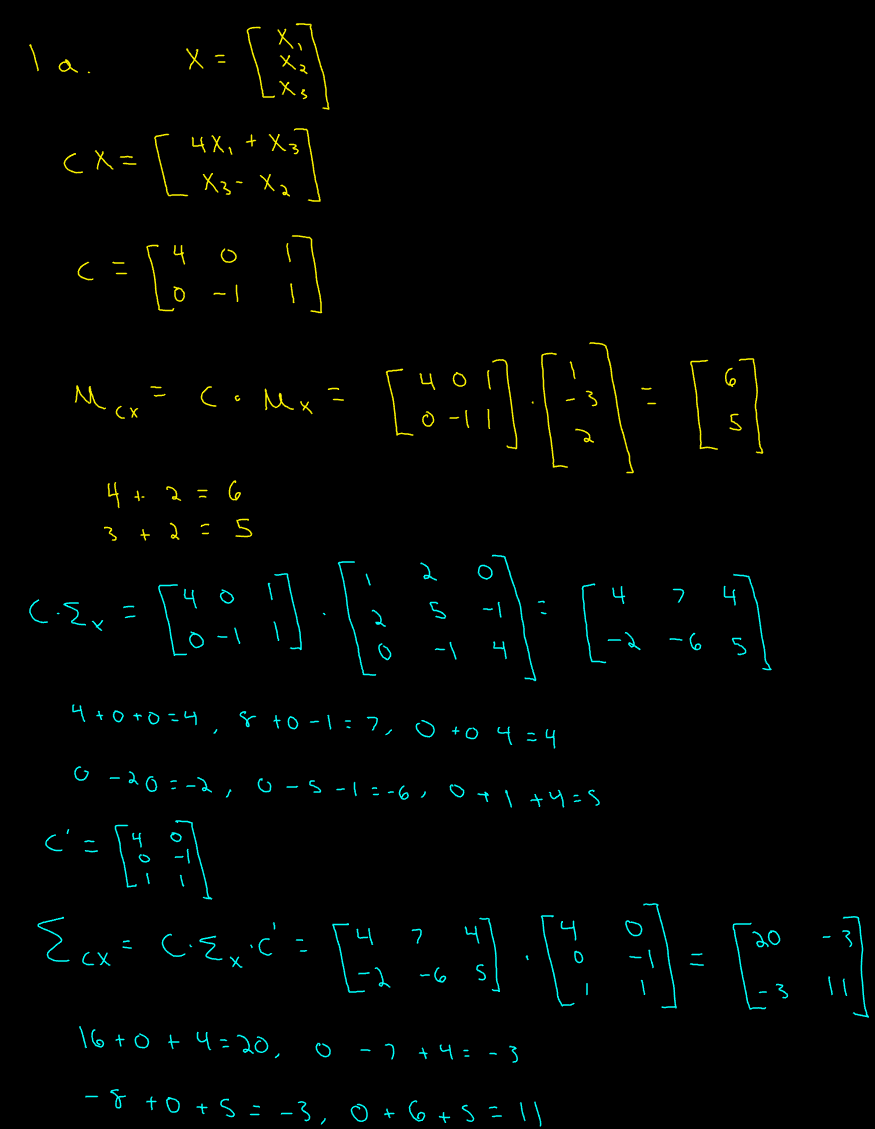
\includegraphics[width=0.6\textwidth]{Selection_1086.png} 
    \caption{Handwritten work for question 1a. }
    \label{fig:handwritten1}
\end{figure}

The coefficient matrix $C$ is:
\[ 
C = \begin{bmatrix} 4 & 0 & 1 \\ 0 & -1 & 1 \end{bmatrix}
\]

The mean vector of the coefficient matrix $\mu_{CX}$ is :

\[ 
\mu_{CX} = \begin{bmatrix} 6 \\ 5\end{bmatrix}
\]

Lastly, the covariance matrix $\Sigma_{CX}$ is:

\[ 
\Sigma_{CX} = \begin{bmatrix} 20 & -3 \\ -3 & 11\end{bmatrix}
\]



        \item Determine which of the following random variables are independent. Justify your answer.\\
        \textit{Hint: having 0 covariance is equivalent to independence for normal random variables}
        \begin{enumerate}[label=\roman*.]
            \item $X_1$ and $X_2$
            \item $X_1$ and $X_3$
            \item $4X_1 + X_3$ and $X_3 - X_2$ \textit{Hint: use your answer above}
        \end{enumerate}
    \end{enumerate}

\begin{figure}[htbp]
    \centering
    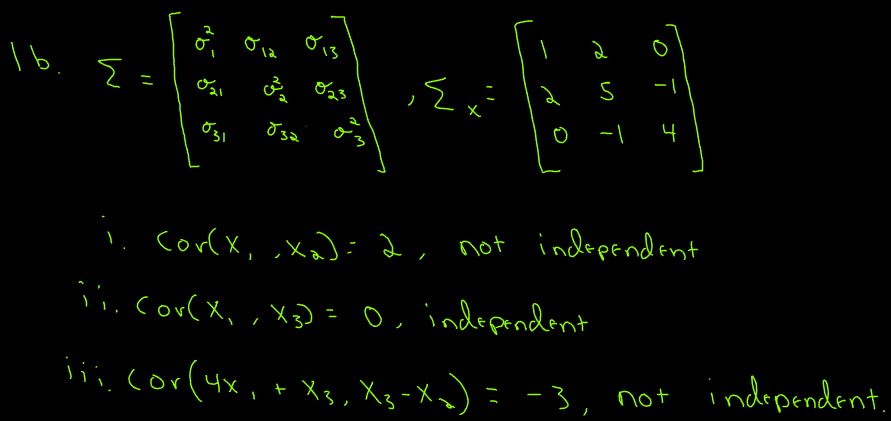
\includegraphics[width=0.6\textwidth]{Selection_1087.png} 
    \caption{Handwritten work for question 1b. }
    \label{fig:handwritten1}
\end{figure}

        \begin{enumerate}[label=\roman*.]
            \item $X_1$ and $X_2$ are dependent since the covariance is 2.
            \item $X_1$ and $X_3$ are independent since the covariance is 0.
            \item $4X_1 + X_3$ and $X_3 - X_2$ are dependent since the covariance is -3
        \end{enumerate}
\pagebreak
    \item (\textit{adapted from J\&W 1.27}) The data in ``parks.csv'' is of attendance (millions) at the fifteen most visited national parks and their size (acres). It can be read into SAS with the commands
    
\begin{verbatim}
data parks;
infile "/parks.csv" firstobs=2 delimiter=",";
input size visitors;
run;
\end{verbatim}

    \begin{enumerate}
        \item Construct a QQ plot relating the squared Mahalanobis distances to the chi-square quantiles. What do you expect this plot to look like if these variables were bivariate normal? Is this a reasonable assumption based on what you see here? Why or why not? \\
        
    Using the following SAS Code:
        
        \begin{verbatim}
proc princomp std out=pcresult;   
var size visitors;   
run;   

data mahal;   
set pcresult;   
dist2=uss(of prin1-prin2); 
run;   

proc print;
var dist2; 
run;   

proc sort;   
by dist2;   
run;   

data plotdata;  
set mahal;
prb=(_n_ -.5)/15;
chiquant=cinv(prb,2);   
run;   

proc gplot;  
plot dist2*chiquant;   
run;
        \end{verbatim}
        
\begin{figure}[htbp]
    \centering
    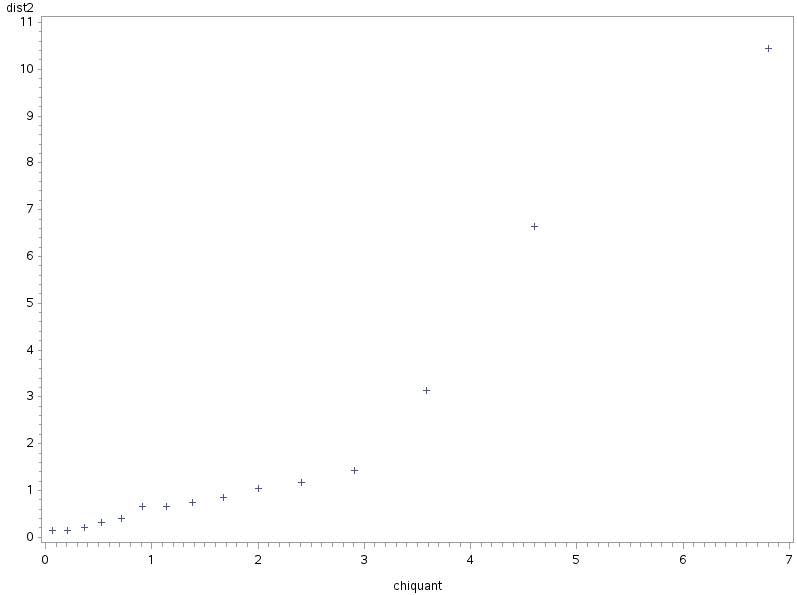
\includegraphics[width=1.0\textwidth]{Selection_1088.png} 
    \caption{SAS output for question 2a. }
    \label{fig:sas1}
\end{figure}

Figure \ref{fig:sas1} depicts the QQ plot that relates the quared Mahalanobis distances to the chi-square quantiles. It is expected that the points would follow a line with a slope of one. However, the points do not follow this trend, for example with the chi-square quant being approximate 7 while the distance is 10.5. \\

\pagebreak
        \item Construct a histogram for each of the variables, and comment on the shape. Are these plots consistent with your observations above? Why or why not?
        
 Using the following SAS Code:
        
        \begin{verbatim}
proc univariate data=parks;
histogram size visitors;
run;
        \end{verbatim}
        
  
\begin{figure}[htbp]
    \centering
    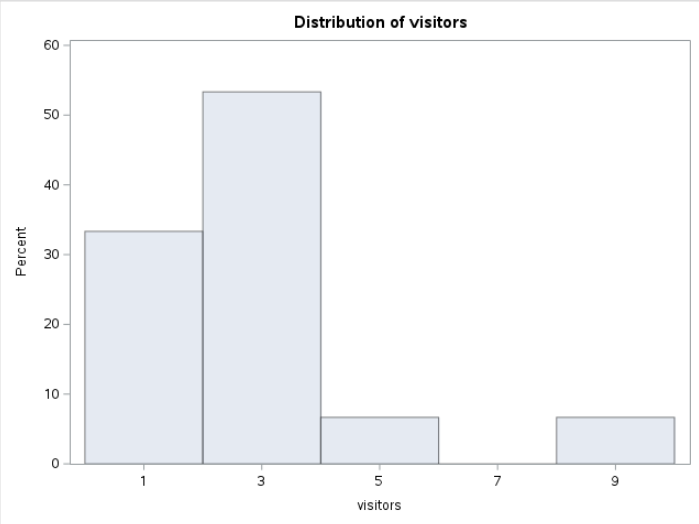
\includegraphics[width=1.0\textwidth]{Selection_1089.png} 
    \caption{SAS output for question 2b(1). }
    \label{fig:sas2}
\end{figure}


\begin{figure}[htbp]
    \centering
    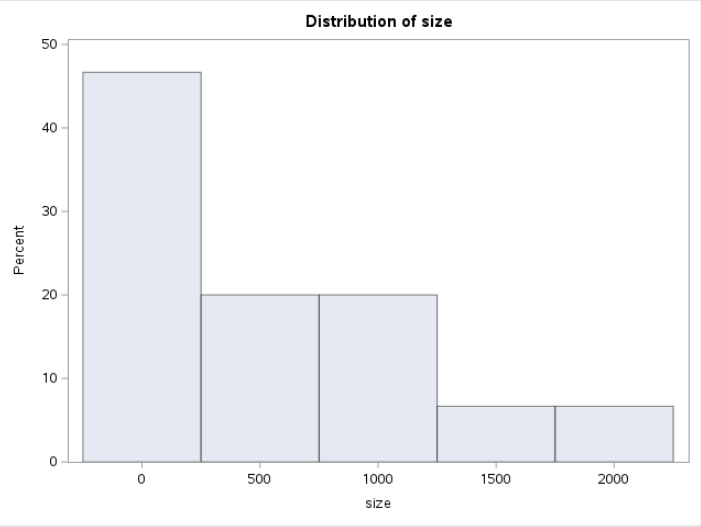
\includegraphics[width=1.0\textwidth]{Selection_1090.png} 
    \caption{SAS output for question 2b(2). }
    \label{fig:sas3}
\end{figure}

        Figures \ref{fig:sas2} and \ref{fig:sas3} depict hisograms of the vistors and size variables. Both variables have a right skew, making it unlikely that they are normally distributed. This finding is consistent with the upward arc seen in Figure \ref{fig:sas1}. \\
        
        \pagebreak
        \item Provide a scatterplot of the two variables. What shape would you expect this plot to have if these variables were bivariate normal? Is this a reasonable assumption based on what you see here? Why or why not? Also, comment on evidence of any outliers.
        
                \begin{verbatim}
proc sgplot data=parks;
    scatter x=size y=visitors;
run;
        \end{verbatim}

\begin{figure}[htbp]
    \centering
    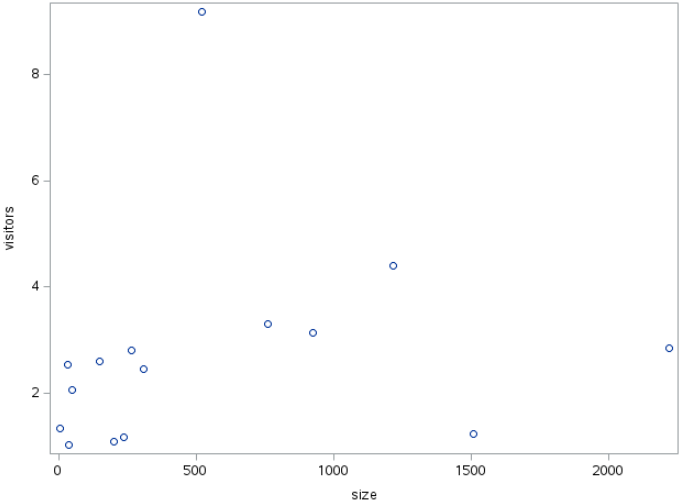
\includegraphics[width=1.0\textwidth]{Selection_1091.png} 
    \caption{SAS output for question 2c. }
    \label{fig:sas4}
\end{figure}

        
        The scatterplot in Figure \ref{fig:sas4} suggests that the two variables are not bivariate normal. It is expected that there would be an ellipse shape formed from the points in the scatter plot if there size and visitors were bivariate normal. Additionally, there are significant outliers, such as a where size exceeds 2000 and the visitors is approximately 2,000 and where the size is 500 and the visitors exceeds 8,000.
        
    \end{enumerate}
\end{enumerate}

\end{document}
